\begin{figure}[ht!]
	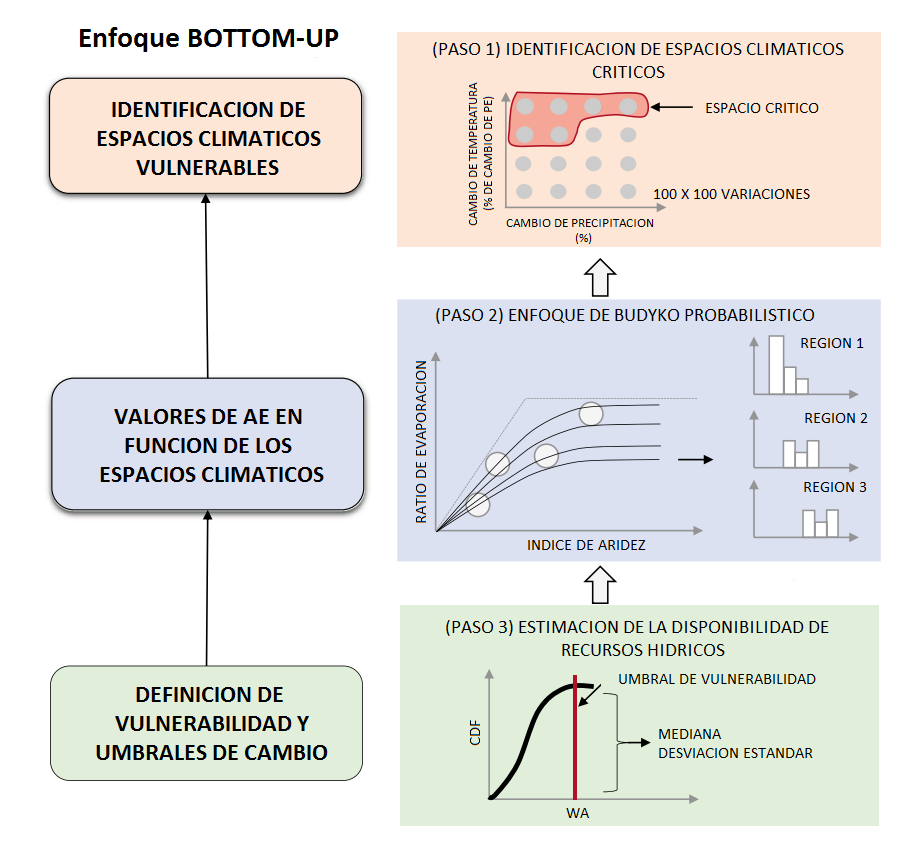
\includegraphics[scale=0.57]{Images/Singh2015.png}
	\centering
	\caption{(Izquierda) Enfoque “bottom-up". (Derecha) Aplicación del enfoque “bottom-up" para evaluar la disponibilidad de los RH en Perú. Selección de los espacios climáticos (paso 1), aplicación del Budyko probabilístico (paso 2) y estimación de la disponibilidad de los RH (paso 3).}
	Fuente: Modificado de \citet{Singh2015}.
	\label{fig:Singh2015}
\end{figure}